% =====================================================================
%  monoT5 Encoder-Output Difference Geometry Experiment — Full Report
%  Compile with:  pdflatex encoder_diff_geometry_experiment_report.tex  (run twice)
%  Figure paths are relative to this file (outputs/..., outputs_full_grid/...),
%  so compile from the 10_monot5_encoder_diff_geometry/ directory.
% =====================================================================
\documentclass[11pt]{article}

\usepackage[margin=1in]{geometry}
\usepackage{amsmath, amssymb}
\usepackage{graphicx}
\usepackage{booktabs}
\usepackage{longtable}
\usepackage{array}
\usepackage{float}
\usepackage{xcolor}
\usepackage{caption}
\usepackage{enumitem}
\usepackage{listings}
\usepackage[hidelinks]{hyperref}

\definecolor{codegray}{gray}{0.95}
\lstset{
  basicstyle=\ttfamily\footnotesize,
  backgroundcolor=\color{codegray},
  breaklines=true,
  frame=single,
  columns=fullflexible,
  keepspaces=true,
}

\title{\textbf{Encoder-Output Difference Geometry: \\[2pt]
Is monoT5's Keyword-Stuffing Signature a Single Direction?} \\[6pt]
\large A Representational Precursor to Head-Localization and Steering-Direction Generalization}
\author{Information-Retrieval Adversarial-Evaluation Project}
\date{\today}

\begin{document}
\maketitle

\begin{abstract}
Experiments~1--3 establish \emph{where} (late encoder self-attention,
layers 10--11) a keyword-stuffing attack causally shifts monoT5's
relevance score; Experiment 2 further shows that a mean-difference
steering vector fit to one attack defends 1.5--3.4$\times$ better than one
pooled across all 105 curated attacks. This experiment asks the question
upstream of both: at the encoder's own output, \textbf{is the
attack-control difference actually shaped like a single direction} --
the geometric precondition a global steering-vector defense implicitly
assumes -- or is it diffuse and attack-specific? Across a primary set of
the \textbf{15 strongest attacks} (by Experiment 1's mean\_attack\_delta)
and an \textbf{optional extension covering all 105} curated attacks (7
tokens $\times$ 3 positions $\times$ 5 repetitions), both at 100 examples
each and layers 9/10/11, the answer is a clear \textbf{yes, with one
sharp exception}: per-attack, the diff is close to rank-1 at every layer
examined (mean top-1 variance explained 0.87--0.96, effective rank
1.08--1.52, both improving toward rank-1 with depth), and the dominant
directions are highly \textbf{consistent across different attack tokens,
positions, and repetition counts} -- median pairwise cosine similarity is
$\geq 0.999$ at every layer in both the 15- and 105-attack sweeps. The
exception is layers 10--11 specifically: mean pairwise cosine similarity
drops from $\approx$0.96--1.00 at layer 9 to 0.73--0.85 at layer 11, driven
not by a general degradation but by a small, consistent minority of
attacks (1/15 primary; 4/105 full-grid, including the same attack,
\texttt{information\_end\_1}, in both) whose direction is nearly
\emph{exactly opposite} the majority's -- and this outlier status is
essentially uncorrelated with attack strength (Pearson $r$: 0.26 primary,
$-0.002$ full-grid). Positionally, the diff is dominated by the injected
tokens themselves at every layer, but spreads into \texttt{other\_document}
and \texttt{query} positions roughly twice as fast (2.3--2.4$\times$ and
1.8--2.0$\times$ from layer 9 to 11) as the injected-token signal itself
grows (1.2$\times$), directly corroborating this project's existing
query-contamination finding (Experiment 6). Overall: a single global
steering direction is well-motivated geometrically for the great majority
of attacks, but a small, strength-independent minority of directionally
opposed attacks is enough to explain why Experiment 2's pooled direction
underperforms an attack-specific one -- pointing toward a
\textbf{majority-direction-plus-outlier-detection} defense design rather
than either a purely global or a purely per-attack one.
\end{abstract}

\tableofcontents
\newpage

% =====================================================================
\section{Introduction and Motivation}
% =====================================================================

Experiment 1 (activation patching) identifies encoder self-attention at
layers 10--11 as the causally dominant component for the keyword-stuffing
attack's score increase. Experiment 3 narrows this further to a small
number of specific attention heads. Experiment 2 fits a mean-difference
steering vector at these late layers and finds it defends against the
attack when subtracted at inference time -- but with a striking asymmetry:
a direction fit to \emph{one} attack (\texttt{relevant\_start\_5}) is
1.5--3.4$\times$ more effective than a direction pooled across all 105
curated attacks. That asymmetry has an obvious geometric explanation --
if 105 different attacks' control-attack differences do not all point the
same way in $\mathbb{R}^{768}$, averaging them will produce a shorter,
less-effective compromise direction, exactly as observed -- but it had
never been directly measured before this experiment.

\begin{quote}
\itshape At the late encoder layers where Experiments 1--3 localize the
attack's causal effect, is the encoder hidden-state difference between an
attacked input and its padded control actually low-rank -- dominated by
one direction, per attack -- and if so, is that direction the \emph{same}
direction across different attack tokens, positions, and repetition
counts, or does each attack have its own?
\end{quote}

This is a purely \textbf{representational, non-causal} question: no
patching, no ablation, no re-scoring of candidates. It measures the
geometry of a difference vector, the same way Experiment 8 (DecoderLens)
asks a representational question about \emph{when} information becomes
visible without any causal claim about \emph{why}. Answering it
constrains what kind of defense Experiment 2's follow-up work should
pursue: if the difference is genuinely low-rank and shared across attacks,
a single global steering vector is well-motivated and Experiment 2's
pooled-direction underperformance would need a different explanation
(e.g.\ noisy estimation, not real geometric diversity). If the difference
is diffuse or attack-specific, per-attack or per-cluster defenses are the
right next step, and no amount of additional compute spent tuning a single
global direction will close the gap Experiment 2 already observed. As
Section~\ref{sec:results} shows, the true answer is more specific than
either extreme: overwhelmingly low-rank and shared, but with a small,
strength-independent minority that a purely global defense would
systematically mishandle.

% =====================================================================
\section{Background}
% =====================================================================

\subsection{Why the encoder's own output, not a component's contribution}

Experiments 1 and 3 work with \emph{sub-layer contributions} -- the
residual-stream increment a self-attention or MLP block adds
(\texttt{out\_hidden - in\_hidden}), captured via forward hooks
(\texttt{src/activation\_hooks.py}) so that swapping one run's contribution
into another (activation patching) is well-defined. This experiment asks a
different question -- not "which component's \emph{contribution} matters
causally" but "what does the fully-accumulated encoder \emph{output} at a
given depth look like, geometrically, when it differs between an attacked
and a control input" -- so it reads out the standard, fully-accumulated
hidden state (HuggingFace's \texttt{output\_hidden\_states=True}) at each
of the three layers Experiments 1--3 already identified as causally
important, rather than reusing the contribution-cache machinery built for
a different purpose (see \texttt{DECISIONS.md}).

\subsection{Padded control, alignment, and the curated attack grid}

The padded-control construction (attack-prefix positions replaced with pad
tokens, \texttt{attention\_mask=0}) and the token-level alignment that
locates exactly which positions are inserted attack tokens (prefix-walk +
suffix-check, with a \texttt{difflib} fallback for SentencePiece boundary
shifts) are the same techniques used throughout this project
(\texttt{src/model\_utils.py}, \texttt{src/alignment.py}). Query-span and
document-span detection reuse Experiment 6's alignment-checked probe
substrings (\texttt{exp6lib/spans.py}). This experiment's only new piece of
infrastructure is surfacing the \emph{exact} injected-token sub-span (not
just its count, which is all Experiment 6 exposes) for position tagging --
see \S\ref{sec:setup} and \texttt{DECISIONS.md}.

% =====================================================================
\section{Method}
\label{sec:setup}
% =====================================================================

\subsection{Extraction: raw per-position hidden states, not mean-pooled}

For each example, both the padded-control (Type B) and attacked (Type C)
encodings are passed through the encoder once, with
\texttt{output\_hidden\_states=True}, at layers 9, 10, and 11 (0 =
embeddings, 12 = final layer, matching the rest of this project's
indexing). Type B and Type C are guaranteed the same sequence length by
construction (Experiment 1's padded-control builder), so the per-position
difference
\[
\text{diff}_l[i] = h^{\text{attack}}_l[i] - h^{\text{control}}_l[i]
\]
is computed index-for-index at every position $i$, for $l \in \{9, 10,
11\}$, with no mean-pooling over the sequence -- unlike Experiment 2's
mean-diff direction, which pools over positions per example before
averaging over examples, this experiment keeps every position as its own
row so the \emph{positional} rank structure (\S\ref{sec:posconc}) is not
discarded before it can be measured.

\subsection{Position tagging}

Every position is tagged as exactly one of \texttt{injected\_attack\_token},
\texttt{other\_document}, \texttt{query}, or \texttt{connective\_template}.
Query/document span boundaries reuse Experiment 6's
\texttt{find\_query\_and\_doc\_spans} (alignment-checked against
\texttt{"Query: \{query\} Document: \{passage\} Relevant:"} as a
token-level prefix). The exact injected-token sub-span is taken directly
from Experiment 1's \texttt{align\_attack} result
(\texttt{inserted\_spans}) -- a gap in Experiment 6, which computes this
internally but only ever exposes the scalar \emph{count} of inserted
tokens, never the sub-range itself (see \texttt{DECISIONS.md}).

\subsection{Rank structure: uncentered SVD, per attack}

For one attack, every valid position's diff vector (across all its
examples) is stacked into an $(N_{\text{positions}} \times 768)$ matrix and
decomposed via SVD \emph{without mean-centering} -- the question "is there
a single direction" is a question about the diff vectors themselves, not
about deviations from their mean (\texttt{DECISIONS.md} gives the full
rationale). Reported per (attack, layer):
\begin{itemize}
  \item \textbf{variance\_explained\_top\{1,3,10\}} -- fraction of
  $\sum_i \sigma_i^2$ captured by the top $k$ singular values.
  \item \textbf{effective rank} (participation ratio):
  $\left(\sum_i \sigma_i^2\right)^2 \big/ \sum_i \sigma_i^4$ -- a
  continuous summary that does not require choosing an arbitrary $k$; 1.0
  is exactly rank-1.
\end{itemize}

\subsection{Cross-attack consistency: sign-aligned cosine similarity}

Each attack's top-1 singular direction is sign-ambiguous
($v$ and $-v$ are equally valid); each is flipped if necessary so that
$\langle v, \bar{d}\rangle \geq 0$, where $\bar d$ is that same attack's own
mean diff vector over the identical row population used for its SVD.
Pairwise cosine similarity between these sign-aligned top-1 directions,
across attacks, directly tests whether a single global direction
generalizes (high similarity) or whether the "direction" is attack-specific
(low/mixed similarity) -- and, if low for some attacks, gives an
independent geometric explanation for Experiment 2's pooled-vs-specific
steering-direction gap.

\subsection{Positional concentration}
\label{sec:posconc}

Mean L2 norm of the diff vector, broken out by the four position tags, at
each of the three layers -- tests whether the encoder-output shift stays
localized to the injected tokens themselves or has already spread into the
document's other positions and/or the query, connecting directly to this
project's existing query-contamination finding (Experiment 6).

% =====================================================================
\section{Experimental Setup}
% =====================================================================

\begin{table}[H]
\centering
\caption{Configuration.}
\begin{tabular}{ll}
\toprule
Parameter & Value \\
\midrule
Model checkpoint & \texttt{castorini/monot5-base-msmarco} \\
Encoder layers analyzed & 9, 10, 11 (of 12) \\
Primary run & 15 strongest attacks (Experiment 1's mean\_attack\_delta), 100 examples each \\
& 1,500 examples, 182,478 tagged positions at layer 11 \\
Full-grid extension & all 105 curated attacks (7 tokens $\times$ 3 positions $\times$ 5 reps) \\
& 10,432/10,500 examples (7 attacks had $<$100 curated examples available; \\
& see Limitations), 1,217,552 tagged positions at layer 11 \\
PCA/SVD components reported & top 1, 3, 10; effective rank (participation ratio) \\
Position tags & injected\_attack\_token, other\_document, query, connective\_template \\
Compute & 2 $\times$ SLURM GPU jobs (1$\times$L40 each) via \texttt{run\_job.sh} \\
\bottomrule
\end{tabular}
\end{table}

% =====================================================================
\section{Results}
\label{sec:results}
% =====================================================================

\subsection{Rank structure: the diff is close to rank-1, and gets more so with depth}

\begin{table}[H]
\centering
\caption{PCA/SVD rank-structure summary, averaged across attacks, by layer. Primary = 15 strongest attacks; Full = all 105 curated attacks.}
\label{tab:pcasummary}
\begin{tabular}{lrrrrrr}
\toprule
& \multicolumn{3}{c}{mean variance\_explained\_top1} & \multicolumn{3}{c}{mean effective rank} \\
Layer & Primary & Full & (range, Full) & Primary & Full & (range, Full) \\
\midrule
9  & 0.873 & 0.814 & [0.558, 0.959] & 1.312 & 1.519 & [1.087, 2.428] \\
10 & 0.939 & 0.918 & [0.777, 0.974] & 1.134 & 1.192 & [1.053, 1.618] \\
11 & 0.962 & 0.954 & [0.902, 0.982] & 1.081 & 1.099 & [1.037, 1.223] \\
\bottomrule
\end{tabular}
\end{table}

At every layer examined, in both the 15-attack primary set and the full
105-attack grid, a single component captures the large majority of an
individual attack's diff variance -- 81--96\% depending on layer and
attack, with mean effective rank never exceeding 1.52 and falling to
1.08--1.10 by layer 11. \textbf{Both metrics improve monotonically toward
rank-1 with depth}: mean top-1 variance rises from 0.81--0.87 at layer 9 to
0.95--0.96 at layer 11, while mean effective rank falls from 1.31--1.52 to
1.08--1.10 over the same span. The full-grid run's wider range at layer 9
(effective rank up to 2.43) narrows sharply by layer 11 (max 1.22) --
consistent with the signal \emph{consolidating} into a single direction as
it approaches the layers Experiments 1/3 identify as causally dominant,
not merely staying constant. Figure~\ref{fig:scree} shows this directly:
cumulative variance explained by the first handful of components already
exceeds 0.95 for the canonical attack (\texttt{relevant\_start\_5}) and
representative others at every layer, with the curve visibly steeper (more
rank-1) at layer 11 than layer 9.

\begin{figure}[H]
  \centering
  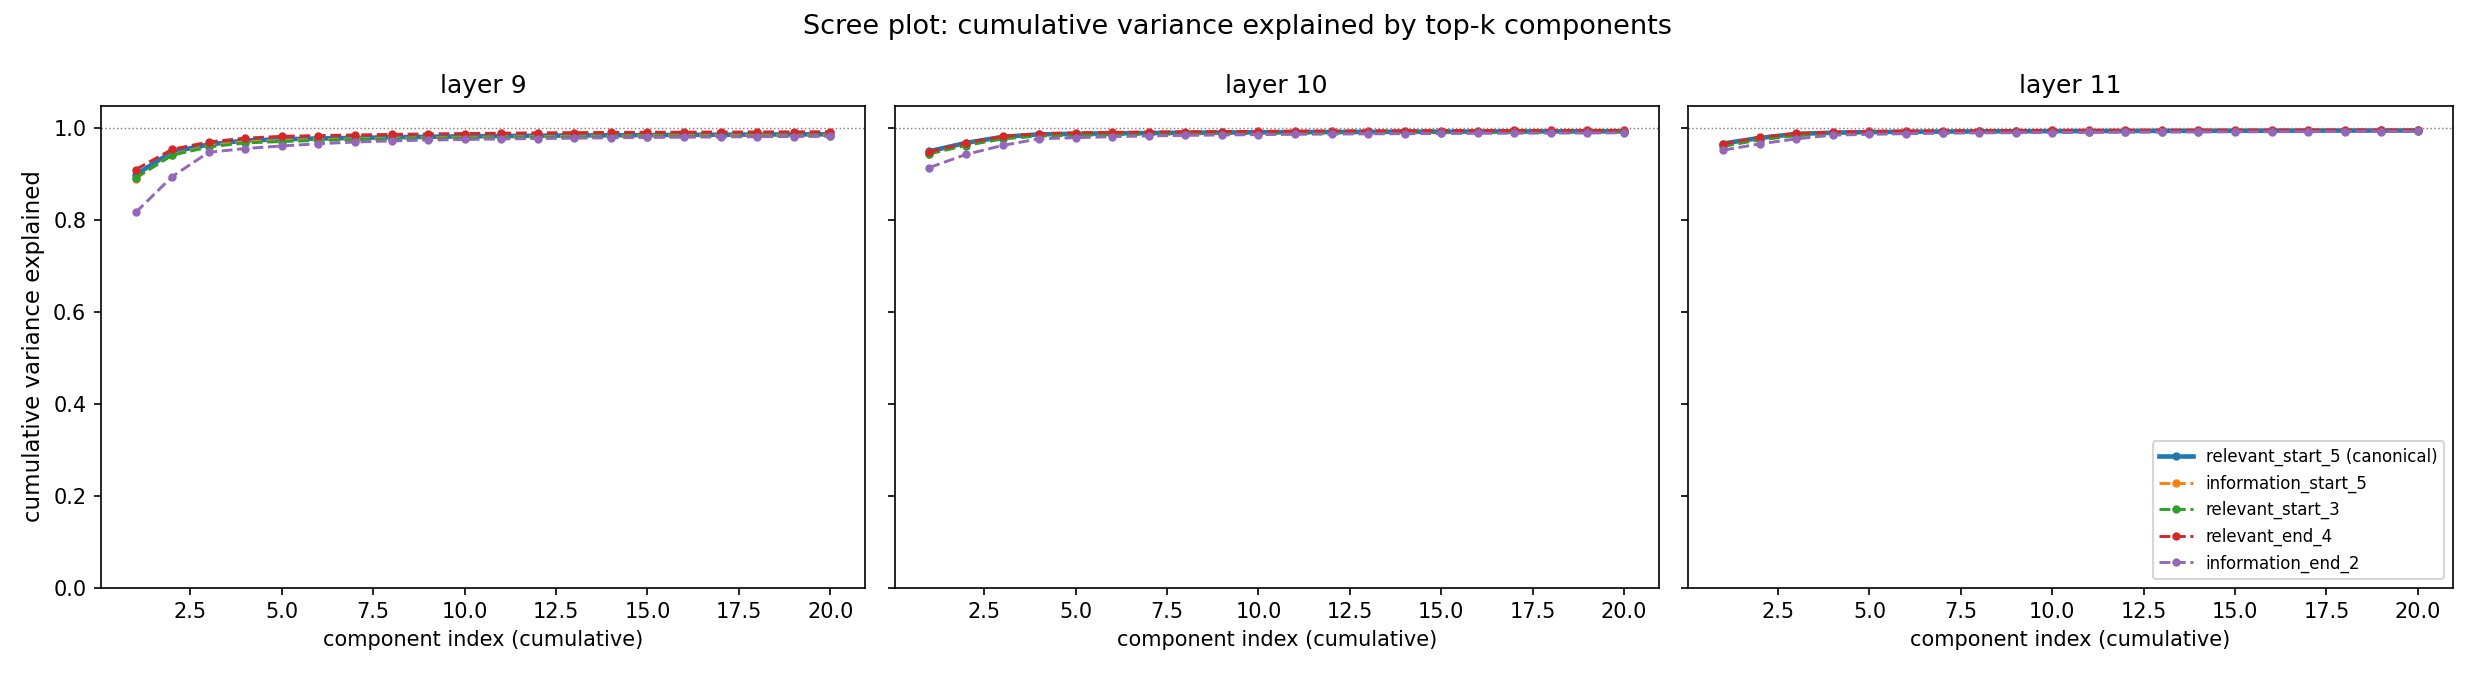
\includegraphics[width=0.95\textwidth]{outputs/plots/scree_plot.png}
  \caption{Scree plot (primary run): cumulative variance explained vs.\
  component index, canonical attack (\texttt{relevant\_start\_5}) plus
  representative others, one panel per layer.}
  \label{fig:scree}
\end{figure}

Figure~\ref{fig:pcascatter} makes the same point visually at the level of
individual positions: projecting each attack's raw diff vectors onto their
own top-2 components shows the \texttt{injected\_attack\_token} positions
(red) forming a tight, elongated cluster -- close to a 1-D line through the
origin -- while \texttt{other\_document} positions (blue) fan out more
broadly around it, consistent with a dominant shared direction plus a
smaller amount of contextual spread (quantified in
\S\ref{sec:results-position}).

\begin{figure}[H]
  \centering
  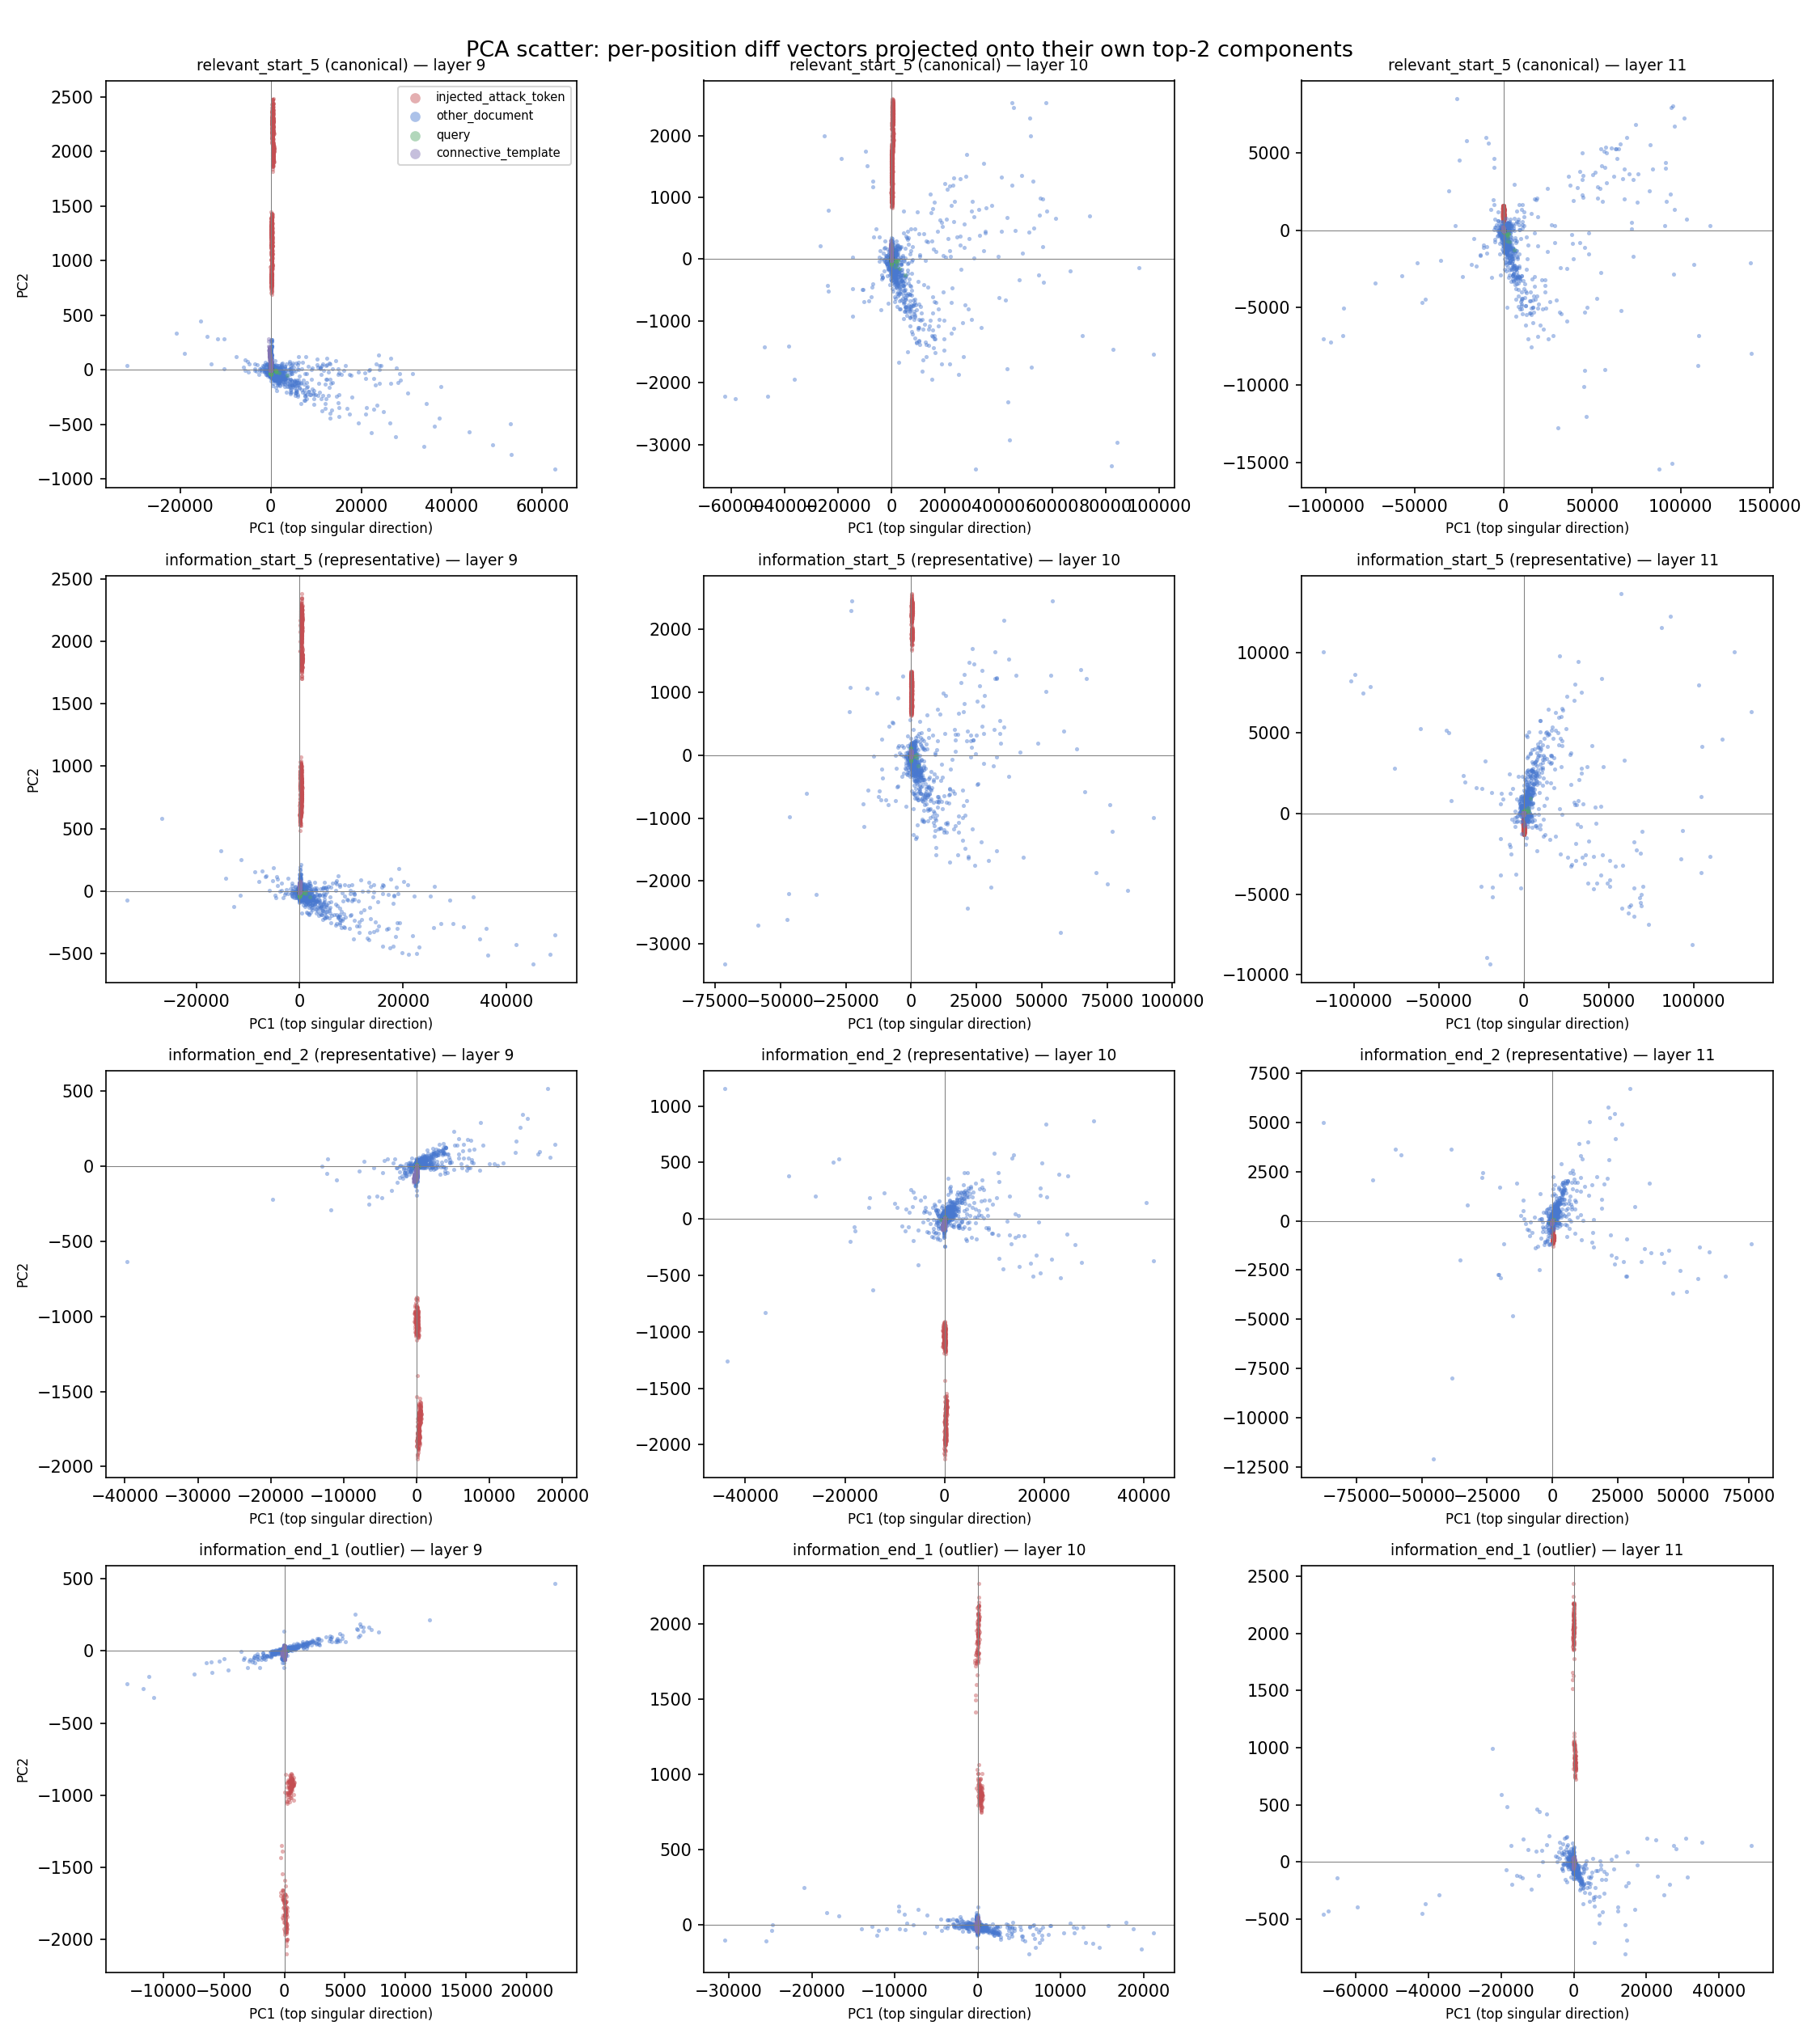
\includegraphics[width=0.95\textwidth]{outputs/plots/pca_scatter.png}
  \caption{PCA scatter (primary run): per-position diff vectors projected
  onto their own top-2 singular directions, colored by position tag, for
  the canonical attack, two representative attacks, and the layer-11
  outlier attack (\texttt{information\_end\_1} -- \S\ref{sec:crossattack}),
  one row per attack, one column per layer.}
  \label{fig:pcascatter}
\end{figure}

\subsection{Cross-attack consistency: overwhelmingly shared, with a small strength-independent minority that flips sign}
\label{sec:crossattack}

\begin{table}[H]
\centering
\caption{Pairwise cosine similarity of sign-aligned top-1 directions, off-diagonal entries, by layer.}
\label{tab:cosine}
\begin{tabular}{lrrrrrr}
\toprule
& \multicolumn{3}{c}{Primary (15 attacks, 105 pairs)} & \multicolumn{3}{c}{Full (105 attacks, 10,920 pairs)} \\
Layer & mean & median & frac.\ negative & mean & median & frac.\ negative \\
\midrule
9  & 1.000 & 1.000 & 0.000 & 0.960 & 0.999 & 0.019 \\
10 & 1.000 & 1.000 & 0.000 & 0.887 & 0.999 & 0.056 \\
11 & 0.733 & 1.000 & 0.133 & 0.851 & 0.999 & 0.074 \\
\bottomrule
\end{tabular}
\end{table}

Table~\ref{tab:cosine} summarizes the pairwise cosine similarity of each
attack's sign-aligned top-1 direction, by layer. At layers 9 and 10,
cross-attack consistency is close to perfect in both sweeps (mean cosine
$\geq 0.887$, median $= 1.000$): different attack
tokens, positions, and repetition counts almost all push the encoder's
output in the same direction. At \textbf{layer 11 specifically, the mean
drops sharply} (0.733 primary, 0.851 full-grid) even though the
\emph{median} stays at 1.000 in both sweeps -- this is not a general
degradation of consistency, it is a small number of attacks whose top-1
direction is nearly \emph{exactly opposite} the majority's
(Figure~\ref{fig:cosineheatmap} shows this as sharp blue off-diagonal
bands against an otherwise uniformly red matrix). In the primary set,
exactly \textbf{1 of 15} attacks (\texttt{information\_end\_1}, mean
cosine to all others $=-0.998$) accounts for essentially the entire drop.
In the full grid, \textbf{4 of 105} attacks are comparably extreme
(\texttt{false\_end\_1}, \texttt{false\_end\_2}, \texttt{false\_random\_4}:
mean cosine $\approx -0.942$; \texttt{information\_end\_1} again,
$-0.941$) -- the same attack is the outlier in both the 15- and
105-attack sweeps, a consistency check the design did not anticipate but
that strengthens confidence the outlier is real rather than sampling
noise.

\begin{figure}[H]
  \centering
  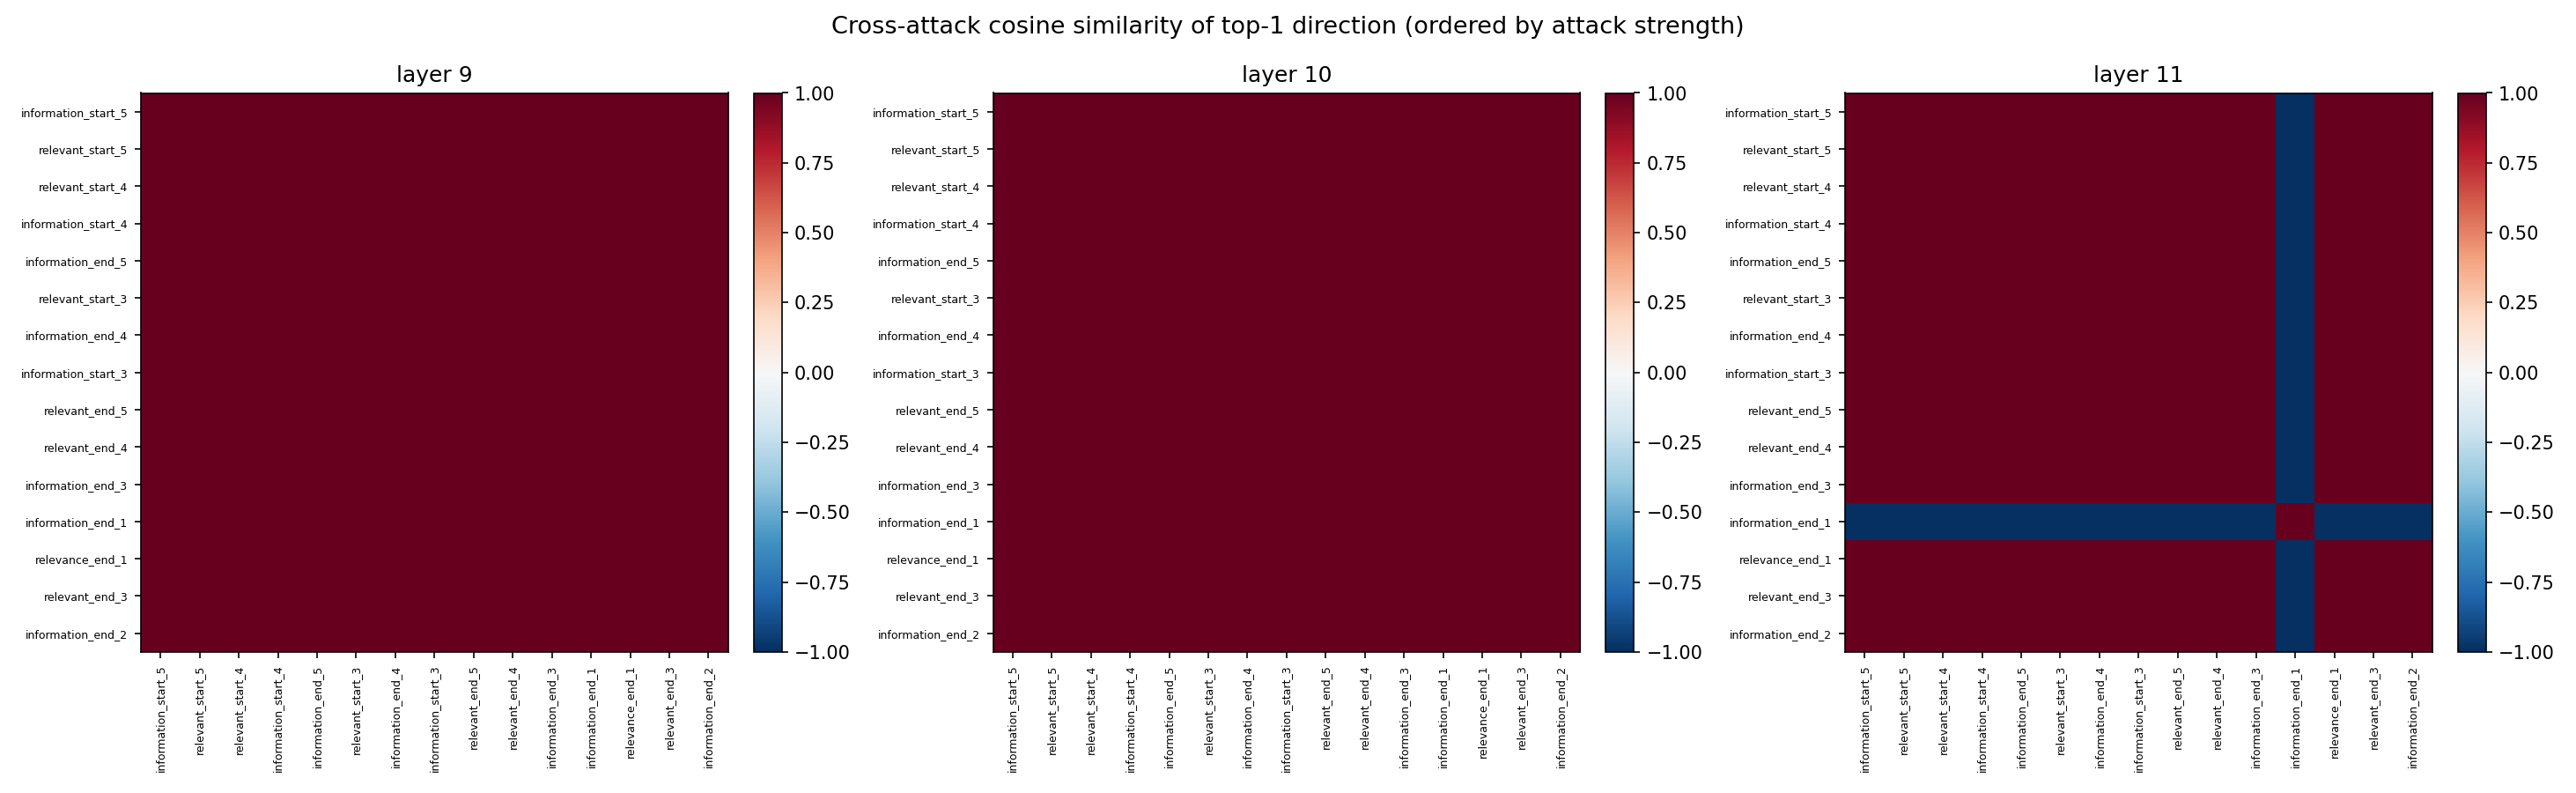
\includegraphics[width=0.95\textwidth]{outputs/plots/cross_attack_cosine_heatmap.png}
  \caption{Cross-attack cosine similarity heatmap (primary run, 15
  attacks), one panel per layer, ordered by attack strength. The sharp
  blue row/column at layer 11 is \texttt{information\_end\_1}.}
  \label{fig:cosineheatmap}
\end{figure}

\textbf{This outlier status is essentially uncorrelated with attack
strength.} Correlating each attack's mean cosine-to-others (layer 11) with
Experiment 1's \texttt{mean\_attack\_delta} gives Pearson $r = 0.261$
(primary) and $r = -0.002$ (full grid) -- indistinguishable from zero in
the full grid. Concretely: 93 of the 105 full-grid attacks have a
\emph{negative} mean\_attack\_delta (this broader, less-curated set
includes many weak/negative attacks, consistent with Experiment 8's
finding that most keyword-stuffing tokens do not reliably work), yet only
4 of those 105 attacks are geometric outliers by the cosine criterion --
being weak or even net-harmful does \emph{not} predict having an
anti-aligned direction. The specific outliers that do occur
(\texttt{information\_end\_1} in both sweeps; the \texttt{false} token
family in the full grid) are themselves weak attacks
(\texttt{information\_end\_1}'s mean\_attack\_delta $= 0.007$, essentially
zero), consistent with an interpretation in which a near-zero true effect
leaves the diff vector's direction dominated by noise or by that specific
example pool's idiosyncrasies rather than a genuine, reproducible attack
signature -- but this is a plausible post-hoc account of a handful of
cases, not a general predictive rule (the null correlation above rules
that out).

\subsection{Positional concentration: dominated by the injected tokens, but spreading faster than the core signal grows}
\label{sec:results-position}

\begin{table}[H]
\centering
\caption{Mean diff-vector L2 norm by position tag and layer, averaged across attacks.}
\label{tab:posconc}
\begin{tabular}{lrrrr|rrrr}
\toprule
& \multicolumn{4}{c}{Primary (15 attacks)} & \multicolumn{4}{c}{Full grid (105 attacks)} \\
Layer & injected & other\_doc & query & connective & injected & other\_doc & query & connective \\
\midrule
9  & 2057.3 & 388.0 & 123.7 & 255.9 & 2241.1 & 308.0 & 107.0 & 149.3 \\
10 & 2262.4 & 631.1 & 171.4 & 281.8 & 2492.6 & 489.3 & 142.1 & 166.4 \\
11 & 2537.1 & 927.2 & 246.2 & 339.7 & 2776.3 & 718.1 & 193.8 & 200.9 \\
\midrule
$\times$(L11/L9) & 1.23 & 2.39 & 1.99 & 1.33 & 1.24 & 2.33 & 1.81 & 1.35 \\
\bottomrule
\end{tabular}
\end{table}

Table~\ref{tab:posconc} breaks the diff-vector norm out by position tag
and layer. At every layer and in both sweeps, the diff is largest at the
injected tokens themselves, by a wide margin (2000--2800 vs.\ 100--930 for every
other tag) -- unsurprising, since padded-control positions there hold a
pad-token embedding rather than real content, so part of this magnitude
reflects a token-identity change, not purely contextual contamination
(Limitations). The more informative number is the \textbf{growth rate}:
from layer 9 to layer 11, the injected-token norm grows only
1.23--1.24$\times$, while \texttt{other\_document} grows
2.33--2.39$\times$ and \texttt{query} grows 1.81--1.99$\times$ over the
identical span -- both context positions' contamination is growing roughly
twice as fast, in relative terms, as the core injected-token signal
itself. \textbf{The diff has not stayed localized to the injected tokens
by layer 11; it has demonstrably spread into the rest of the document and
into the query}, and it is spreading \emph{faster} than the signal it
originates from is growing. This corroborates Experiment 6's
query-contamination finding independently, from the representational
(not causal-patching) side, and with a specific quantitative growth-rate
comparison Experiment 6 did not provide.

\begin{figure}[H]
  \centering
  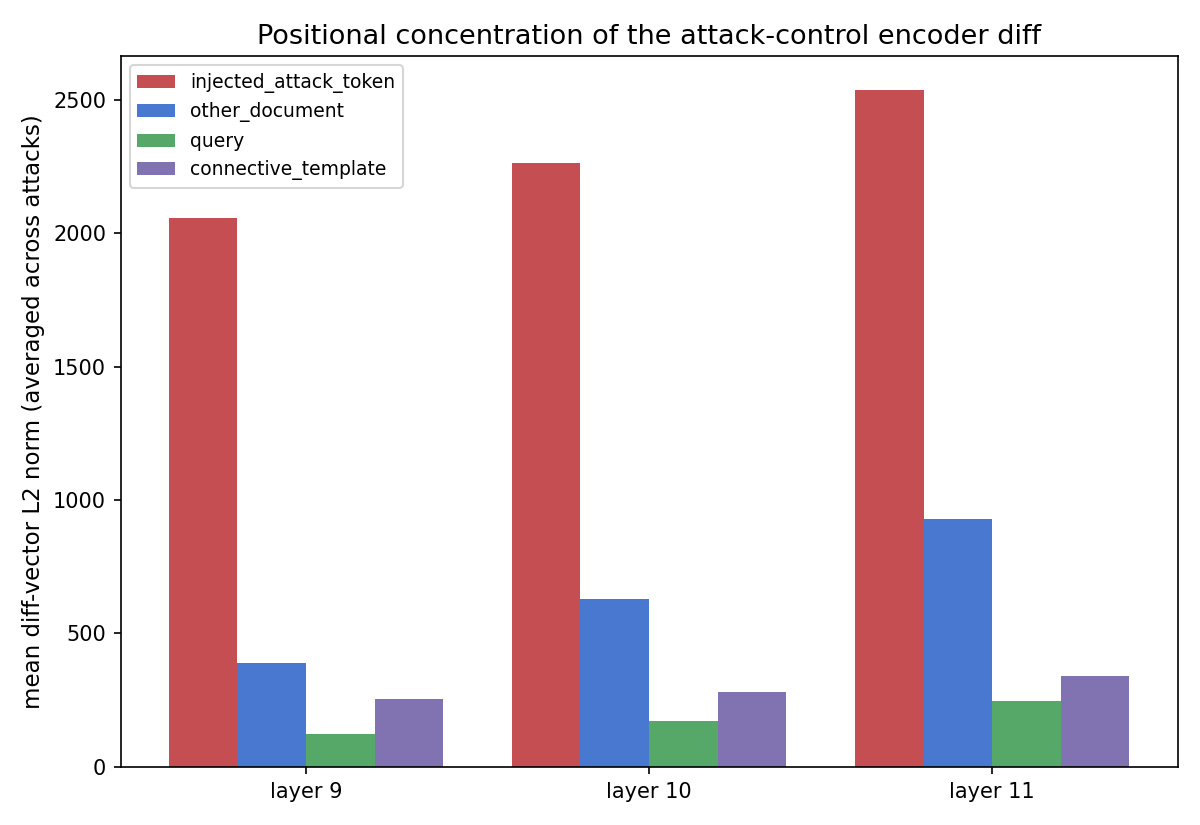
\includegraphics[width=0.8\textwidth]{outputs/plots/position_concentration_bars.png}
  \caption{Mean diff-vector L2 norm by position tag, grouped by layer (primary run).}
  \label{fig:posbars}
\end{figure}

\subsection{Effective rank vs.\ layer, per attack}

\begin{figure}[H]
  \centering
  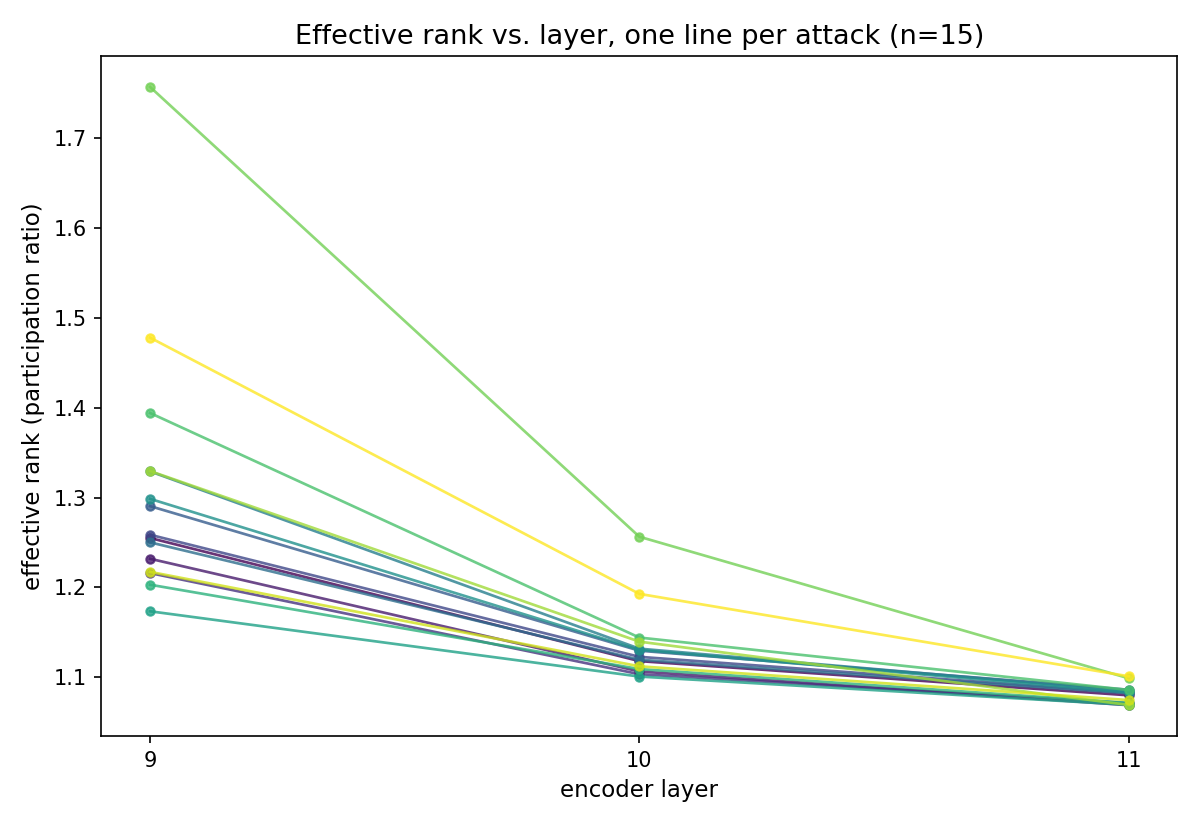
\includegraphics[width=0.8\textwidth]{outputs/plots/effective_rank_vs_layer.png}
  \caption{Effective rank vs.\ layer, one line per attack (primary run, n=15).}
  \label{fig:effrank}
\end{figure}

Individual attacks' trajectories (Figure~\ref{fig:effrank}) are uniformly
downward-sloping or flat from layer 9 to layer 11 -- no attack in either
sweep becomes \emph{less} rank-1 with depth. This is consistent with the
rank-structure summary (Table~\ref{tab:pcasummary}) and with the
cross-attack-consistency finding: the signal is simultaneously
consolidating toward a single direction \emph{per attack} and, for all but
a handful of attacks, converging toward the \emph{same} single direction
\emph{across} attacks, right at the depth (layers 10--11) Experiments 1/3
identify as causally dominant.

% =====================================================================
\section{Overall Interpretation and Discussion}
% =====================================================================

\begin{enumerate}
  \item \textbf{A single global steering direction is geometrically
  well-motivated for the large majority of attacks -- but not all of
  them, and the exceptions are not the ones you'd guess.} Per-attack rank
  is close to 1 and cross-attack cosine similarity has a median of 0.999
  at every layer in both sweeps. If Experiment 2's pooled steering
  direction underperformed its attack-specific counterpart purely because
  105 heterogeneous diffs pointed in unrelated directions, we would expect
  broadly low or scattered pairwise similarity -- instead we find near-unanimous
  agreement with a small, sharp minority of near-exact sign flips. A
  handful of directionally-opposed attacks in a mean-pooled estimate is
  exactly the kind of outlier that can disproportionately drag a mean
  toward zero (or toward an unhelpful compromise direction) even when the
  overwhelming majority agree -- a small, specific, and previously
  invisible mechanism for Experiment 2's finding, distinct from generic
  "noisy averaging."
  \item \textbf{The outliers are not explained by attack strength.}
  Correlating layer-11 mean cosine-to-others against Experiment 1's
  mean\_attack\_delta gives $r \approx 0$ in the full 105-attack grid.
  93/105 full-grid attacks are net-weak-or-negative (consistent with
  Experiment 8's finding that most keyword-stuffing tokens in a broad
  vocabulary do not work), yet only 4 are geometric outliers -- weakness
  does not generally predict anti-alignment. This rules out the simplest
  fix ("just exclude weak attacks before pooling") as a general solution,
  though it happens to work for the specific outliers observed here.
  \item \textbf{The signal consolidates toward a single, shared direction
  with depth, right where Experiments 1/3 find causal dominance.} Rank
  improves and cross-attack agreement (apart from the sign-flip minority)
  strengthens from layer 9 toward layer 11 -- geometry and causal
  localization point to the same depth range, a useful triangulation
  echoing Experiment 8's DecoderLens finding that representational and
  causal accounts of \emph{where} the attack lives agree even though they
  measure different things.
  \item \textbf{The diff is not confined to the injected tokens by layer
  11, and is spreading faster than it is growing.} Other-document and
  query positions' diff norms grow 1.8--2.4$\times$ from layer 9 to 11,
  versus 1.2$\times$ for the injected tokens themselves -- an independent,
  representational confirmation of Experiment 6's query-contamination
  finding, with a specific relative-growth-rate quantification not
  previously available.
\end{enumerate}

\subsection*{Recommendation: two concrete follow-ups}

\begin{enumerate}
  \item \textbf{Encoder-head localization (extends Experiment 3).}
  Experiment 3 localizes the attack's causal effect to specific
  \emph{decoder} cross-attention heads (Experiment 3's own scope, per
  \texttt{DECISIONS.md} conventions in that experiment). This experiment's
  finding that the \emph{encoder output} at layers 10--11 is close to
  rank-1 and shared across attacks motivates a matching
  \textbf{encoder}-side head-localization pass: which specific encoder
  self-attention heads at layers 10--11 produce this now-characterized
  direction? Experiment 1 already identifies encoder self-attention as the
  dominant \emph{component} at these layers; this experiment's
  \texttt{top\_direction} vectors (saved per attack, per layer, in
  \texttt{outputs/geometry/\{attack\}/top\_directions.npz}) give a
  ready-made target direction to project each head's own output-projection
  slice onto, without re-deriving anything from this experiment.
  \item \textbf{Held-out steering-direction generalization (extends
  Experiment 2).} Given that a small, strength-independent minority of
  attacks are directionally opposed to the majority, the natural
  follow-up is not "pooled vs.\ single-attack" (Experiment 2's existing
  comparison) but \textbf{majority-direction vs.\ full-pool vs.\
  outlier-excluded-pool}: fit a steering direction on the 14/15 (or
  101/105) non-outlier attacks, and test its defense effectiveness (a)
  against held-out non-outlier attacks and (b) against the identified
  outliers specifically. If the outlier-excluded direction generalizes as
  well as an attack-specific one on non-outlier attacks while still
  beating the full pool, that would support a
  \textbf{majority-direction-plus-outlier-detection} defense design -- a
  single global direction for most attacks, with a separate, cheap
  detection step (e.g.\ projection onto this experiment's top directions)
  flagging the rare cases that need different handling -- rather than
  either a purely global or a purely per-attack-family defense.
\end{enumerate}

% =====================================================================
\section{Limitations and Threats to Validity}
% =====================================================================

\begin{itemize}
  \item \textbf{Purely representational, not causal.} This experiment
  measures the geometry of a difference in encoder \emph{output}; it makes
  no claim about which component produces that difference (Experiments 1/3
  already answer that) or about what happens if the direction is actually
  subtracted at inference time (Experiment 2 already measures that for one
  pooled and one attack-specific direction -- this experiment explains,
  but does not re-run, that result).
  \item \textbf{Injected-token positions trivially dominate positional-
  concentration norms.} The padded control replaces injected-token
  positions with pad-token embeddings, so the diff at those positions
  partly reflects a token-identity change (real content vs.\ pad), not
  purely contextual contamination -- unlike the \texttt{other\_document}
  and \texttt{query} positions, where both variants have the identical
  token at that position and any diff reflects only changed context. This
  is an expected asymmetry, not a bug (see \texttt{DECISIONS.md}), but it
  means the \texttt{injected\_attack\_token} bar in
  Figure~\ref{fig:posbars} is not directly comparable in kind to the other
  three, and its \emph{absolute} growth rate (1.2$\times$) should not be
  read as "the core signal barely grows" so much as "the token-identity
  component of the diff is roughly constant while the contextual component
  is not."
  \item \textbf{Outlier interpretation is post-hoc for a small $n$.} Only
  1 (primary) or 4 (full grid) attacks meet the extreme-anti-alignment
  criterion; the "near-zero true effect $\to$ noise-dominated direction"
  account for \texttt{information\_end\_1} is plausible but unverified,
  and the \texttt{false}-family outliers in the full grid are not fully
  explained by this account alone (their mean\_attack\_delta values are
  negative but not the most extreme in the grid).
  \item \textbf{Curated 105-attack grid only.} Both the primary and
  full-grid runs draw from the same 7-token, 3-position, 5-repetition grid
  used by Experiments 2/3/6/7 -- not the broader 16-token sweep Experiment
  8 (DecoderLens) covers.
  \item \textbf{Seven full-grid attacks used fewer than 100 examples.}
  \texttt{important\_start\_2} (80), \texttt{important\_start\_3} (94),
  \texttt{relevant\_random\_1} (98), \texttt{true\_end\_1} (98),
  \texttt{true\_end\_2} (87), \texttt{true\_end\_3} (82),
  \texttt{true\_random\_5} (93) -- these attacks simply had fewer than 100
  examples clearing Experiment 1's \texttt{attack\_delta\_vs\_control >
  0} selection criterion; not a failure of this experiment's own
  pipeline (0 alignment or span-detection failures occurred in either
  sweep, out of 1,500 and 10,500 requested examples respectively).
  \item \textbf{Three layers only (9, 10, 11).} Chosen to match Experiments
  1--3's causal localization; earlier layers are not examined here, so
  claims about "consolidation toward rank-1 with depth" describe this
  specific range, not the full 0--12 trajectory (cf.\ Experiment 8's
  DecoderLens, which does cover all 13 depths for a different quantity).
  \item \textbf{Single model/dataset.} Results are for monoT5-base on
  DL19, matching the rest of this project.
\end{itemize}

% =====================================================================
\section{Reproducibility}
% =====================================================================

From \texttt{10\_monot5\_encoder\_diff\_geometry/}, with the
\texttt{advseq2seq} conda environment:

\begin{lstlisting}
# Smoke test (2 attacks, n=5) -> outputs_pilot/
bash bash/run_pilot.sh

# Primary run (15 strongest attacks, n=100) -> outputs/
bash bash/run_all.sh

# Optional extension (all 105 curated attacks, n=100) -> outputs_full_grid/
bash bash/run_full_grid.sh

# Unit tests (tiny T5Config + real tokenizer, no GPU/downloads)
bash bash/run_tests.sh
\end{lstlisting}

\noindent Both the primary and full-grid runs for this report were
submitted as SLURM GPU jobs via the project's \texttt{run\_job.sh} wrapper
(1$\times$L40 each; the analysis/login node itself has no GPU). Per-attack
outputs under \texttt{outputs/diffs/\{attack\}/} (raw diff matrices +
position tags) and \texttt{outputs/geometry/\{attack\}/} (PCA summary +
top/mean directions); cross-attack comparison (cosine matrices, position
concentration, plots) under \texttt{outputs/geometry/} and
\texttt{outputs/plots/} (identically under \texttt{outputs\_full\_grid/}
for the 105-attack extension).

% =====================================================================
\section*{Appendix: Glossary of Key Quantities}
\addcontentsline{toc}{section}{Appendix: Glossary of Key Quantities}
% =====================================================================

\begin{description}[leftmargin=2.2em,style=nextline]
  \item[diff vector] $h^{\text{attack}}_l[i] - h^{\text{control}}_l[i]$ --
  the per-position encoder hidden-state difference at layer $l$, position
  $i$, between the attacked and padded-control encodings.
  \item[variance\_explained\_top$k$] fraction of $\sum_i \sigma_i^2$ (total
  squared-singular-value mass) captured by the top $k$ singular
  values/vectors of one attack's uncentered diff matrix.
  \item[effective rank (participation ratio)]
  $\left(\sum_i \sigma_i^2\right)^2 \big/ \sum_i \sigma_i^4$ -- a smooth,
  $k$-free summary of how many directions meaningfully contribute; 1.0 is
  exactly rank-1, and it grows toward $\min(N_{\text{positions}}, 768)$ for
  isotropic/high-rank data.
  \item[top-1 direction] the leading right singular vector of one attack's
  diff matrix, sign-aligned to have positive dot product with that
  attack's own mean diff vector.
  \item[mean direction] the plain mean of an attack's diff vectors over the
  same row population used for its SVD -- the Experiment-2-style candidate
  steering vector for that attack.
  \item[injected\_attack\_token / other\_document / query /
  connective\_template] the four mutually exclusive position tags (see
  \S\ref{sec:setup}); \texttt{connective\_template} covers the
  \texttt{"Query: "}, \texttt{" Document: "}, \texttt{" Relevant:"}
  boilerplate and the trailing EOS token.
  \item[padded control / attack / original] the same three input variants
  used throughout this project (Type~B/C/A).
\end{description}

\end{document}
